\chapter{Jednání parlamentu jako trénovací data}
\label{kap:svolocz}

Trénovacích dat pro rozpoznávání řeči není nikdy dost. V~době psaní tohoto textu
je manuálně přepsaných asi 100 hodin z~Mluveného korpusu Karla Makoně. To je pro
natrénování modelu pro jednoho mluvčího použitelné množství. Zda by více trénovacích dat od jiných mluvčích mohlo pomoci, je však
otevřená otázka.

Veřejně k~dispozici je několik zdrojů trénovacích dat pro účely trénování
rozpoznávače češtiny, jichž jsem si vědom:
\begin{itemize}
\item{
    Vystadial\cite{vystadialarticle} se 77 hodinami záznamů internetových
    rozhovorů\cite{vystadialdata},
}
\item{
    The Prague Database of Spoken Czech\cite{pdtscarticle} se 122 hodinami
    spontánních dialogů anotovaných na několika úrovních\cite{pdtscdata},
}
\item{
    Korpus expresivní mluvy COMPANION s~5 hodinami namluvenými jednou
    profesionální mluvčí\cite{companiondata},
}
\item{
    Otázky Václava Moravce: 35 hodin přepsaných záznamů české talk
    show\cite{ovmdata},
}
\item{
    STAZKA: 35 hodin záznamů z~vozidel na silnicích obsahujících anotované
    promluvy\cite{stazkadata},
}
\item{
    88 hodin automaticky přepsaných záznamů z~jednání poslanecké
    sněmovny\cite{pspdata}.
}
\end{itemize}
Celkem se tak dostaneme přibližně na 350 hodin dalších trénovacích dat.

Ze záznamů jednání poslanecké sněmovny však existují také ruční stenografické
přepisy. Velká část jednání a jejich přepisů je veřejně ke stažení na webových
stránkách poslanecké sněmovny. Pokusil jsem se proto z~těchto dat připravit
korpus pro trénování rozpoznávání řeči.

\section{Příprava dat}

Ruční přepisy jednání poslanecké sněmovny jsou, pokud je mi známo, k~dispozici
pouze ve formátu čitelném pro člověka. Přepisy nejsou ve zdrojovém kódu webové
stránky nijak oddělené a jsou promíchané s~metainformacemi. Je tedy nutné
extrakci pojmout jako aproximační úkol. Používám velice jednoduchý algoritmus,
který má své nedostatky, ale pokrývá drtivou většinu záznamů. Extrahuji podstrom
všech elementů s~hodnotou atributu \texttt{[align=justify]} vyjma elementů
\texttt{<b>}, neboť ty obsahují jména mluvčích.

Známé nedostatky spočívají jednak v~tom, že se jména mluvčích sice správně z~přepisu
oddělují, ale navzdory jejich hodnotě coby metainformace zahazují, a jednak
v~tom, že se z~přepisu vynechávají odkazy na jiné schůze. Ty jsou totiž
formátované jinak než ostatní části, jak je vidět např. v~přepisu schůze z 12.
února 2020 od
10:10\footnote{https://www.psp.cz/eknih/2017ps/stenprot/040schuz/s040372.htm}.
Opravení obého je otázkou napsání chytřejšího scraperu a pro účely vybudování
korpusu pro tréning rozpoznávání řeči je obé bezvýznamné: Označení mluvčích
z~principu, vynechání odkazů pro jejich řídkost.

\subsection{Zarovnávání}
\label{subsec:svolocz:zarovnavani}

Jedna z~překážek použití stenografických přepisu pro trénování rozpoznávačů řeči
je velmi volné párování neboli zarovnání přepisů ke zvuku. Každý zvukový záznam
má 14 minut a překrývá se se sousedními čtyři minuty na každé straně.
Přepisy jsou rozdělené na úseky odpovídající těmto záznamům. Zarovnání je tedy
do desetiminutových bloků s~dvouminutovým přesahem na každé straně. Na
obrázku~\ref{fig:svolocz:overlap} je vyobrazeno schéma tohoto apriorního
zarovnání.

\begin{figure}[htpb]
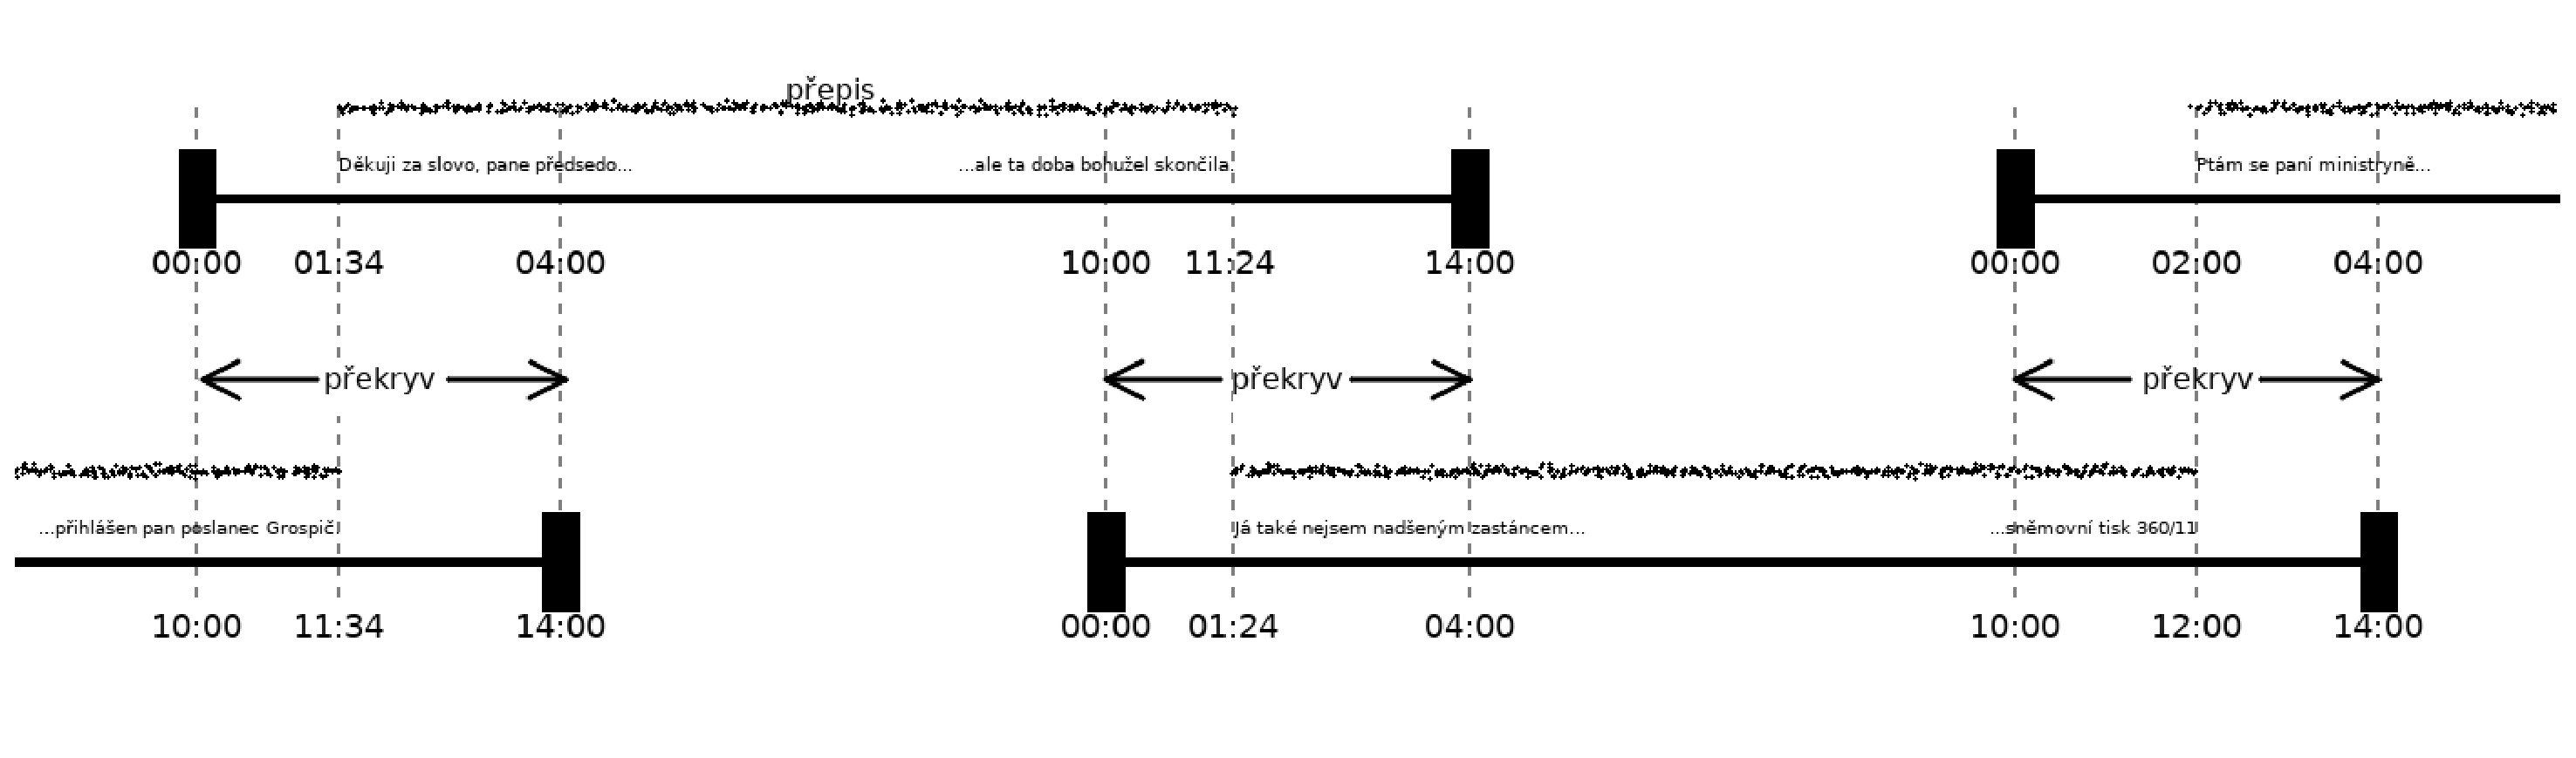
\includegraphics[scale=0.25]{rc/svolocz-overlap.eps}
\caption{Apriorní zarovnání a překryv zvukových záznamů k~přepisům. Vyobrazen je
záznam z 12. února 2020 kolem 10. hodiny. Přepis záznamu vlevo nahoře pokrývá
pozice od 01:34 do 11:24. Vpravo dole pak od 01:24 do 12:00.}
\label{fig:svolocz:overlap}
\end{figure}

Systémů pro zarovnávání dlouhých zvukových záznamů existuje několik, publikovali
je např. Moreno et al\cite{moreno1998recursive} nebo
Hazen\cite{hazen2006automatic}. Oba jsou založeny na využití předem získaného a
zarovnaného automatického přepisu. Taktéž tento přistup využívám, ale
zjednodušený a přizpůsobený úloze.

Za použití výše zmíněného datasetu\cite{pspdata} jsem natrénoval markovovský
akustický model obdobný tomu, jenž je popsán v~kapitole~\ref{kap:asr}. Jazykový
model jsem natrénoval ze stažených stenografických přepisů. Těch je podstatně
víc než nahrávek, protože z~mně neznámého důvodu je valná část odkazů na zvukové
záznamy nefunkčních, končíc chybovým kódem 404 nebo v~menším počtu případů 403.

Pro celý korpus jsem pomocí programu julius vygeneroval automatický přepis se
zarovnáním. Automaticky vygenerovaný zarovnaný přepis každého záznamu jsem pak
porovnal s~odovídajícím manuálním přepisem pomocí Levenshteinovy metody počítání
editačních operací. Zjistil jsem samotné editační operace pro přechod
z~automatického přepisu k~manuálnímu a pro každé slovo v~automatickém přepisu
spočetl, kolik úprav naň připadá. Na základě toho definuji pro každé automaticky
vygenerované slovo spolehlivost párování se slovem manuálně zapsaným jako
\begin{equation}1 - \frac{e(w)}{l(w)}\end{equation}
kde $e(w)$ je počet editačních operací nad slovem $w$ a $l(w)$ je délka slova
$w$ v~písmenech.

Obrázek~\ref{fig:svolocz:align} proces zarovnání manuálních přepisů se zvukovým
záznamem zachycuje.

\begin{figure}[htpb]
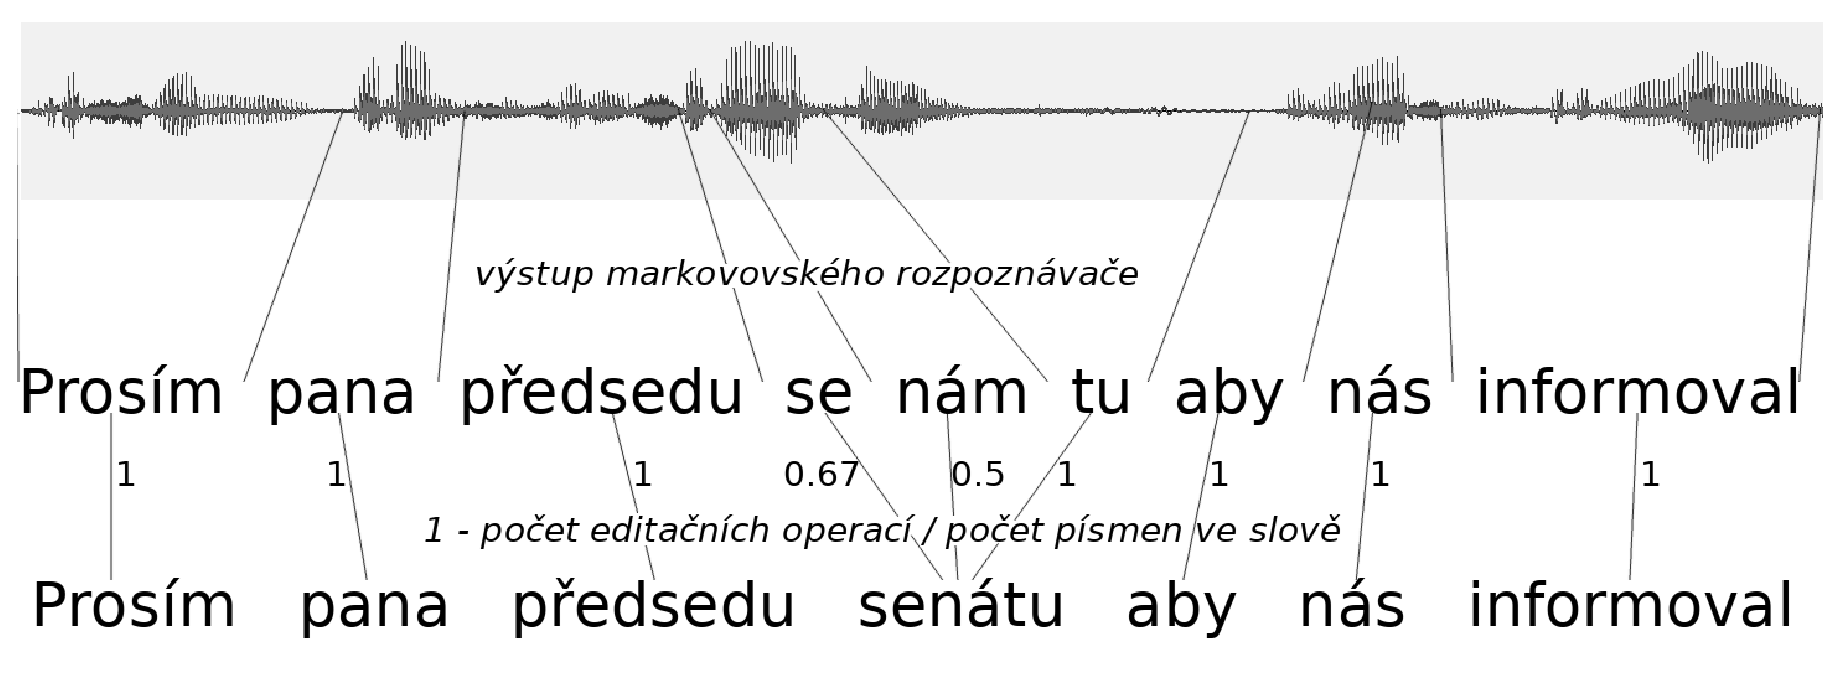
\includegraphics[scale=0.4]{rc/svolocz-align.eps}
\caption{schéma zarovnání zvukových záznamů ke stenografickým přepisům na úrovni
slov}
\label{fig:svolocz:align}
\end{figure}

\subsection{Tvorba potenciálních trénovacích vzorků}

Kvalita trénovacích dat pro rozpoznávání řeči závisí i na tom, jak jsou
rozdělena. Za prvé je žádoucí, aby byly trénovací vzorky podobně dlouhé
jako testovací vzorky\cite{nagorski2003search}.
V~případě automatického přepisu korpusu Karla Makoně lze
nastavit délku vstupních úseků libovolně. V~obecném případě nelze předvídat.
Za druhé je pro tréning výhodné, aby jednotlivé vzorky měly podobnou délku kvůli
efektivnímu využití operační paměti grafické procesní jednotky. Stačí jeden
dlouhý vzorek a dávka {\em (batch)} způsobí vyčerpání paměti. Naopak mnoho
kraťoučkých vzorků způsobí, že se paměť při dávce zaplní jen málo a plýtvá se
časem. Za třetí, chci-li, aby byla trénovací sada dala použitelná i pro ostatní,
je dobré, aby se délkou vzorků příliš neodlišovala od ostatních datových sad.

Nad to je ale důležité, aby přepis dokonale odpovídal obsahu. A protože
vyřezáváme trénovací vzorky z~delších souborů, při čemž může dojít
k~nepřesnostem, je záhodno volit místa řezu tak, aby padla pokud možno do
delších pauz v~řeči. Je to týž problém jako v~sekci~\ref{sec:segmenty}, kde je
podrobně popsán. V~tomto
případě jsem dospěl k~hranicím 12 - 30 sekund a data tak rozdělil na úseky o
délce v~tomto rozpětí.

\subsection{Výběr trénovacích vzorků}

Po rozdělení desetiminutových nahrávek na úseky vhodné délkou pro trénink je
nutné spárovat tyto úseky s~odpovídajícími úseky manuálních přepisů, a ty, které
jsou spárovány spolehlivě, zařadit do samotné trénovací množiny.
V~podsekci~\ref{subsec:svolocz:zarovnavani} jsem popsal, že máme párování
jednotlivých slov v~automatickém a manuálním přepisu s~určitou mírou
spolehlivosti a že automatický přepis je spárován se zvukovým záznamem. Zbývá
tedy vybrat úseky, které můžeme považovat za spolehlivě přepsané, a zbytek
zahodit.

Nahrávky se překrývají tak, že z~každého čtrnáctiminutového souboru je jen deset
minut pokryto odpovídajícím přepisem, takže zahodit musíme minimálně 40\% úseků.
Dospěl jsem k~následujícím kritériím:

\begin{enumerate}
\item{Spolehlivost prvního a posledního slova v~úseku alespoň 70\%.}
\item{Průměrná spolehlivost všech slov v~úseku alespoň 70\%.}
\item{Alespoň 5 slov v~úseku.}
\end{enumerate}

Důvodem k~zahrnutí kritéria minimální spolehlivosti krajních slov je záměr
zajistit správné hranice úseku. Druhé kritérium počítá s~průměrnou spolehlivostí
a ne třeba s~minimem, protože je přípustné, aby některá slova měla i nulovou
spolehlivost, tedy aby v~nich všechna písmena byla špatně. Iniciální přepis
obsahuje mnoho chyb, to je také důvod, proč se trénuje s~manuálním přepisem a ne
s~automatickým. Je-li ale příliš mnoho slov spárováno nespolehlivě, roste šance,
že spárování je skutečně liché. Počet slov v~úseku je mezi kritérii proto, že
u~malého počtu slov je vysoká šance náhody, při které je chybně určeno vysoké
skóre spolehlivosti nesprávně spárovaným slovům.

Ještě vyvstává otázka, proč použít průměr a ne medián spolehlivosti v~druhém
kritériu. Je to z~toho důvodu, že liší-li se výrazně počet slov v~manuálním a
automatickém přepisu, projeví se to jako mnoho operací přidání či smazání
písmene odpovídající jednomu slovu v~automatickém přepisu. V~takovém případě
mohou všechna slova mít stoprocentní spolehlivost, jen jedno hluboce pod nulou.
Takový úsek by pak byl při použití mediánu přijat, zatímco průměr výrazně negativní
hodnotu započte a úsek správně odmítne.

\subsection{Shrnutí extrakce trénovacích dat}

Konstanty a algoritmy použité při extrakci trénovacích dat ze záznamů jednání
Parlamentu České republiky jsou jen hrubě zvoleny a je velký prostor pro jejich
odladění. Vedou ale už teď k~velmi kvalitní datové sadě o velikosti 1058 hodin.
Z~celkového počtu 539~057 úseků jich bylo 142~530 (26\%) zahrnuto do trénovací
sady. Z~celkového počtu 396~527 zavržených úseků jich 350~258 (88\%) bylo
zavrženo kvůli nespolehlivým hraničním slovům. Toto kritérium je však aplikováno
jako první, takže je v~tomto čísle zahrnuto i mnoho úseků, které by jinak byly
odmítnuty některým dalším kritériem.

Sníží-li se potřebná spolehlivost ze 70\% a 50\%, zvýší se počet přijatých úseků
o 17\%. Přidá se tak 5\% úseků z~celkového počtu. Pokud však započteme fakt, že
40\% úseků je nutně odstraněno kvůli překryvům, je celkový přírůstek ve
skutečnosti 9\% celkového počtu. Je to možnost, jak zvýšit objem trénovacích dat
za cenu zvýšení počtu úseků se špatně určenými hranicemi.

\section{Číslovky a zkratky}

Číselných výrazů je v~parlamentních přepisech mnoho. Představují 489~880
ze~25~010~269 tokenů v~kompletním stenografickém přepisu, to jsou téměř dvě
procenta. Ve výše popsaných trénovacích datech je aspoň jedno číslo ve 24\%
vzorků.

Původní moje řešení spočívalo v~zahrnutí číslic do abecedy a tedy
v~pokusu o přepis číselných výrazů přímo na číslice. V~systému rozpoznávání řeči
natrénovaném na těchto datech, popsaném v~následující sekci, bohužel výsledkem bylo, že
číselné výrazy se vždy přepsaly na prázdný řetězec.

K~problému se lze postavit čtyřmi způsoby:
\begin{enumerate}
\item{ignorovat ho,}
\item{vyřadit číslice z~trénovacích dat,}
\item{manuálně číslice rozepsat do slov,}
\item{číslice rozepsat automaticky.}
\end{enumerate}

První možnost ignorování problému asi netřeba rozebírat.
Vyřazení vět s~číslicemi je snadný a použitelný přístup, ale byla by škoda
přijít o čtvrtinu trénovacích dat a o drtivou většinu příkladů číslovek.
Manuální přepis by byl jistě ideální, ale vzhledem k~objemu dat pro mne
nerealizovatelný.

Pro automatický rozpis číslic do slov lze využít hotového aparátu: iniciálního
přepisu a algoritmu pro zarovnávání se stenografickým přepisem.

Rozpis provádím ve dvou krocích:
\begin{enumerate}
\item{vygenerování možných čtení číslicového výrazu,}
\item{výběr nejpravděpodobnější varianty.}
\end{enumerate}

Pro generování možných čtení čísel jsem vyšel z~algoritmu použitého v~modulu pro
Perl \texttt{Lingua::CS::Num2Word}, který jsem doplnil o řád miliard pro
kardinální číslovky, rozšířil tak, aby se místo jedné varianty generovaly
pokud možno všechny gramaticky přípustné, a zahrnul podporu genitivu a
akuzativu, decimálních a ordinálních číslovek, dat a hodin.

Ve stenografických přepisech před dalším zpracováním rozvedu všechny tokeny
obsahující číslice do variant rozpisu a při zarovnávání s~iniciálním
automatickým přepisem vyberu tu variantu, která má nejmenší editační vzdálenost.

Spolu s~číslicemi expanduji také zkratky a symboly. Např. velmi častý symbol
paragraf (§) rozepisuji do variant {\em paragraf, paragrafu, paragrafů,
paragrafem, paragrafech}, které se podle iniciálního přepisu vyskytují jako
jediné časté. Dalšími častými zkratkami s~různými variantami rozpisu jsou {čl. -- článek,
odst. -- odstavec, tzv. -- takzvaný}.

Po provedení expanze se podobnost stenografického a iniciálního automatického
přepisu zvýšila, což se odrazilo i na zvýšení počtu přijatých úseků z~26\% na
35\%. Množství trénovacích dat v~hodinách vzrostlo o 86, tedy na 1144.

\section{Rozpoznávání řeči na různých sadách}
\label{sec:csasr:results}

Výše popsanou datovou sadu jsem použil pro natrénování rozpoznávače řeči pomocí
systému DeepSpeech, stejně jako to popisuju v~kapitole~\ref{kap:asr}. Sadu jsem
rozdělil na trénovací (train), ladicí (dev) a testovací (test) v~poměru 18:1:1.
Hyperparametry jsem nastavil následovně: learning rate 0,0001, dropout rate 0,2,
zbytek ponechán defaultně. Ke konvergenci došlo po 12 epochách. Výsledná WER
byla 8,40\% s~použitím pentagramového jazykového modelu natrénovaného na
stenografických přepisech.

Ze zdrojů zmíněných v~úvodu této kapitoly se bez větší námahy se ziskem v~řádu
aspoň desítek hodin daly použít 1) Otázky Václava Moravce a 2) Vystadial. Krom
toho jsem použil veřejně nepřístupné zdroje 3) CUCFN -- Korpus Finančních zpráv
Univerzity Karlovy, 4) Korpus reprezentativní mluvené češtiny
Oral2013\cite{oral2013} a 5) amatérsky namluvenou Bibli dostupnou z~adresy
\texttt{poslouchamebibli.cz}, u které není žádná explicitní licence.

Na všech sadách včetně manuálních přepisů nahrávek Karla Makoně jsem natrénoval
model s~použitím téhož systému Mozilla DeepSpeech, týchž hyperparametrů a téhož
obecného jazykového modelu. Ten jsem natrénoval na datech z~WMT
2019\cite{wmt19}.

Nakonec jsem natrénoval akustický model na všech trénovacích
sadách sloučených do jedné.
Tabulka~\ref{tab:csasr:results} shrnuje word error rate systémů trénovaných na
jednotlivých částech testovaných jednak na testovací sadě z~téhož zdroje a
jednak na agregované testovací sadě sloučené ze všech dílčích.
Z~důvodu použití obecného jazykového modelu je u parlamentního korpusu vyšší chybovost než
výše zmiňovaných 8,40\% a u Makoňova korpusu taktéž vyšší chybovost než 19\%
uvedených v~sekci~\ref{sec:deepspeech}.

\begin{table}[htpb]
\begin{center}
\begin{tabular}{|l||r|r|}
\hline
zdroj     & WER na sobě & WER na všech \\
\hline
bible     & 9,20\%  & 94,7\% \\
cucfn     & 31,6\%  & 72,8\% \\
makoň     & 30,4\%  & 77,3\% \\
oral2013  & 78,4\%  & 60,7\% \\
ovm       & 21,6\%  & 72,9\% \\
parlament s~číslicemi & 8,74\%  & 39,7\% \\
parlament ve slovech  & 7,89\%  & 36,0\% \\
vystadial & 51,0\%  & 74,0\% \\
\hline
vše s~číslicemi   & 28,4\%  & 28,4\% \\
vše ve slovech    & 26,0\%  & 26,0\% \\
\hline
\end{tabular}
\caption{Word error rate rozpoznávání řeči na jednotlivých korpusech a na jejich
konkatenaci.}\label{tab:csasr:results}
\end{center}
\end{table}

%           cstest      selftest
% ovm       0.728954    0.216131
% bible     0.947226    0.091958
% cucfgn    0.728446    0.316287
% vystadial 0.739838    0.509930
% svolocz   0.397490    0.083978
% makon     0.773216    0.191772
% oral2013  0.607015    0.783525
% all       0.283574    0.283574
%
% cucfgnOF  0.683059    0.141142
% all\o                 0.130555
